%!TEX program = xelatex
\documentclass[11pt,fleqn,twoside]{article}
\usepackage{makeidx}
\makeindex
\usepackage{plain} %bibliography style
\usepackage{amsmath} %math fonts - just in case
\usepackage{amsfonts} %math fonts
\usepackage{amssymb} %math fonts
\usepackage{lastpage} %for footer page numbers
\usepackage{fancyhdr} %header and footer package
\usepackage{mmpv2}
\usepackage{url}
\usepackage{xltxtra}

\usepackage[hidelinks]{hyperref}
	\urlstyle{same}

\usepackage[font=small]{caption}

\usepackage{setspace}
	\setstretch{1.1}

\setmainfont[Ligatures=TeX]{Adobe Garamond Pro}


% the following packages are used for citations - You only need to include one.
%
% Use the cite package if you are using the numeric style (e.g. IEEEannot).
% Use the natbib package if you are using the author-date style (e.g. authordate2annot).
% Only use one of these and comment out the other one.
\usepackage{cite}
%\usepackage{natbib}

\begin{document}

\name{David Field}
\userid{\fontspec[Numbers={OldStyle}]{Adobe Garamond Pro}dvf9}
\projecttitle{Browser-based Online Multiplayer Roleplaying Game}
\projecttitlememoir{Browser-based Online Multiplayer Roleplaying Game} %same as the project title or abridged version for page header
\reporttitle{Outline Project Specification}
\version{1.0}
\docstatus{Final}
\modulecode{CS39440}
\degreeschemecode{G401}
\degreeschemename{Computer Science}
\supervisor{Hannah Dee} % e.g. Neil Taylor
\supervisorid{\fontspec[Numbers={OldStyle}]{Adobe Garamond Pro}hmd1}
\wordcount{}

%optional - comment out next line to use current date for the document
%\documentdate{10th February 2014}
\mmp

\setcounter{tocdepth}{3} %set required number of level in table of contents


%==============================================================================
\section{Project description}
%==============================================================================

\begin{figure}
\centering
	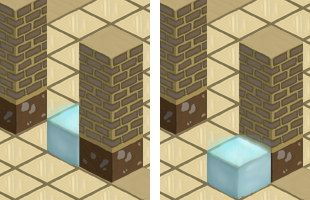
\includegraphics[scale=0.7]{figures/figure-1.png}
	\caption{This image shows a very early build of the game with \textsc{2d} isometric graphics \cite{GameArt}. The blue block represents a player. On the left, the player is obscured by an object; on the right, the player is in front of it.\label{figure_1}}
\end{figure}

An online, multiplayer game based in the browser, utilising \textsc{html5} canvas and JavaScript for the client and Python for the server. It will be played similarly to the table-top roleplaying game \textit{Dungeons \& Dragons}, with a Game Master and several players.

The players will interact with the world in two modes or states. The first is a free-roaming state that operates in real-time. In this state, players will be allowed to interact with the world and the objects and characters within it with relative freedom. The rules that govern them will be loose and mostly describe the interactions of objects with other objects. For example, a magic spell that creates fire would have a heat attribute, and a door made of wood would have a burning point attribute. When they met, if the heat was greater than the burning point, the door would be set on fire.

The other state is the combat state. Players in this state will be locked into a turn-based system where they can only move and perform actions in a limited amount during their turn. Opponents can be creatures or other characters—both player and non-player—and will take their own turns to perform actions. Non-player characters and creatures will be operated by the Game Master. All characters and creatures will have attributes, such as health and mana (for magic), as well as a set of abilities that they can perform. If a character or creature reaches zero health it will have been killed and removed as an active element.

Each player will operate a single character and their view of the world and abilities within it will be defined by that character's location and abilities. If a character is too far away to see another character, then the player will also not see the other character. If a character cannot use magic spells, then the player will not be able to use them.

Player characters who are killed, either in battle or in some other way (perhaps they are killed by falling rocks in the free-roam state) are no longer playable. Players who lose their character may be removed from the game, become a spectator, be given an already existing character previously controlled by the Game Master or be allowed to make a new character.

The Game Master is not a player but rather the controller of the world. They will be able to interact with the world without limitations and be responsible for creating the world via a map editor, guiding the players around it, operating non-player characters and creatures in the world and set up events for the players. The Game Master will even be able to override the normal rules of the world. In the example of the fire spell and the door, the Game Master will be able to say that the door is not set on fire, even if it otherwise would have been.

The world will be presented to users using tile-based, \textsc{2d} isometric graphics (as seen in Figure \ref{figure_1}). It will consist of a planar terrain with objects, items and characters on top of it. Movement in the world will be done in 8 directions: up, down, left, right and diagonal. Characters and creatures will move from tile to tile, with only one able to be in a tile at any given time. However, each tile can hold many items (such as weapons, money, clothes). Objects will be varied, with those such as walls and pillars taking up a tile by themselves but objects such as chairs or chests of treasure that can be interacted with by characters may coexist in a tile with characters.

The players and Game Master will be able to communicate throught a textual chat system. In its most basic form, this will be a global chat that all users in the game can see. However, the ability to restrict chat to a local context or to an individual user would be nice.

Extra features that would enhance the project but are not mandatory include: voice chat system; multi-levelled maps with varying heights; random map generator; random creature/character generator; visual representation for character items (such as weapons, clothes, etc); and the ability for users to upload their own artwork for use in their games.

Development progress can be followed at \url{http://whatproject.tumblr.com/} .

%==============================================================================
\section{Proposed tasks}
%==============================================================================
My proposed tasks to achieve a basic version of the project are as follows:

\begin{itemize}
	\item{Create basic client-side graphics engine, allowing a map to be rendered and a player to move around.}
	\item{Create basic multiplayer functionality, setting up the server and allowing multiple players to exist in the same map and move around within it.}
	\item{Add Game Master, who can select different characters to control.}
	\item{Add items and attributes to characters, allowing them to carry things and setting things up for the next task.}
	\item{Add combat state, allowing users to do more than walk around the world.}
	\item{Add attribute interactions in the free-roam state, allowing for the fire spell and wooden door interaction.}
	\item{Add map editor for the Game Master.}
\end{itemize}

%==============================================================================
\section{Project deliverables}
%==============================================================================
\begin{description}
	\item{\textbf{Game Client,} final `production' version.} This is what the users of the game will interact with, via a browser, allowing for both regular players and a Game Master, who is given the ability to create maps for the game.

	\item{\textbf{Game Server,} final `production' version.} This will be responsible for syncing the game between all the players and providing authoritative state to clients to help prevent cheating.

	\item{\textbf{Documentation.}} Basic guides for users that instruct them on how to operate the game from the Game Master and player perspectives.

	\item{\textbf{Final Report.}} Report detailing the system; the process of the system's creation from beginning to end; differences between the proposal and final system and explanations for those differences; full bibliography.
\end{description}


%
% Start to comment out / remove the following lines. They are only provided for instruction for this example template.  You don't need the following section title, because it will be added as part of the bibliography section.
%
%==============================================================================
% \section*{Your Bibliography - REMOVE this title and text for final version}
% %==============================================================================
% %
% You need to include an annotated bibliography. This should list all relevant web pages, books, journals etc. that you have consulted in researching your project. Each reference should include an annotation.

% The purpose of the section is to understand what sources you are looking at.  A correctly formatted list of items and annotations is sufficient. You might go further and make use of bibliographic tools, e.g. BibTeX in a LaTeX document, could be used to provide citations, for example \cite{NumericalRecipes} \cite{MarksPaper} \cite[99-101]{FailBlog} \cite{kittenpic_ref}.  The bibliographic tools are not a requirement, but you are welcome to use them.

% You can remove the above {\em Your Bibliography} section heading because it will be added in by the renewcommand which is part of the bibliography. The correct annotated bibliography information is provided below.
%
% End of comment out / remove the lines. They are only provided for instruction for this example template.
%


\nocite{*} % include everything from the bibliography, irrespective of whether it has been referenced.

% the following line is included so that the bibliography is also shown in the table of contents. There is the possibility that this is added to the previous page for the bibliography. To address this, a newline is added so that it appears on the first page for the bibliography.
\newpage
\addcontentsline{toc}{section}{Annotated Bibliography}

%
% example of including an annotated bibliography. The current style is an author date one. If you want to change, comment out the line and uncomment the subsequent line. You should also modify the packages included at the top (see the notes earlier in the file) and then trash your aux files and re-run.
%\bibliographystyle{authordate2annot}
\bibliographystyle{IEEEannot}
\renewcommand{\refname}{Annotated Bibliography}  % if you put text into the final {} on this line, you will get an extra title, e.g. References. This isn't necessary for the outline project specification.
\bibliography{mmp} % References file

\end{document}
